\section{Generalizzazione}
	In seguito all'esordio di blockchain assieme a Bitcoin sono state presentate numerose proposte per sviluppi ed implementazioni della tecnologia. Nel seguito di questa sezione si presenta quello che vuole essere uno schema delle caratteristiche salienti di un sistema basato su blockchain: sono riportati le principali scelte di progettazione che lo caratterizzano e alcune delle soluzioni ad oggi adottate. La ricerca è estremamente attiva a riguardo, perciò questo elenco non sarà e non vuole essere esaustivo: lo scopo è quello di chiarire a che tipologie di sistema si fa riferimento parlando genericamente di \emph{blockchain}.
	\subsection{Definizione tecnica}
		Una buona definizione generica di blockchain è quella proposta da Imran Bashir in \emph{Mastering blockchain} \cite{mastering_blockchain}: essenzialmente si tratta di un registro distribuito peer-to-peer, crittograficamente sicuro, append-only, immutabile (o meglio, estremamente difficile da modificare) e aggiornabile solo previo consenso da parte dei peer. Esistono ovviamente molte altre definizioni, ciascuna con enfasi diversa sui vari aspetti di blockchain, tuttavia l'estrema sintesi di quella di Bashir permette di concentrarsi sugli aspetti imprescindibili che la caratterizzano, lasciando alle scelte di progettazione successive il compito di determinarne i particolari.
	
	\subsection{Elementi costitutivi di una blockchain}
		\subsubsection{Permessi di accesso}
			La prima grande suddivisione in macro categorie dei sistemi basati su blockchain ne riguarda le modalità di accesso. La blockchain può essere:
			\begin{itemize}
				\item \textbf{Pubblica} nel momento in cui il sistema è aperto al pubblico e chiunque può installarne un client, scaricare il registro e partecipare attivamente ai processi di validazione dei blocchi. Tipicamente ogni utente scarica e mantiene una copia locale del registro e tramite un sistema di consenso distribuito si raggiunge un accordo con il resto della rete sull'effettivo stato ``ufficiale" dei dati. Tipicamente si affidano ad algoritmi di consenso basati su proof-of-work o proof-of-stake. Sono anche dette \emph{permissionless ledgers}, e l'esempio più noto è Bitcoin;
				\item \textbf{Privata} nel caso l'accesso sia ristretto ad un limitato insieme di utenti o organizzazioni che abbiano deciso di condividere dei registri comuni. In questa accezione di blockchain acquista importanza l'autenticazione degli utenti, e si ottiene una maggiore riservatezza dei dati a costo di rinunciare alla natura completamente ``\emph{trustless}" delle blockchain pubbliche. Ciò porta a differenze sostanziali nella gestione del consenso: è possibile prescindere da prove onerose come la proof-of-work, e soprattutto viene a mancare la necessità di rendere vantaggioso a ciascun peer il mantenimento del sistema.
				Il grado di chiusura di questo tipo di blockchain può variare anche molto: è possibile ad esempio permettere a ciascun utente di osservare il registro ma limitarne ad un insieme ristretto la modifica. Sono anche dette \emph{permissioned ledgers} e esempi possibili sono Ripple e i sistemi costruiti su Hyperledger.
			\end{itemize}
		
		\subsubsection{Meccanismi di consenso}
			La tipologia di consenso adottata caratterizza fortemente l'intero sistema blockchain, ed è strettamente legata alla tipologia di accesso scelta.
			\begin{itemize}
				\item \textbf{Proof of work}: è il meccanismo di consenso adottato da Bitcoin. Richiede la soluzione ad un problema matematico computazionalmente impegnativo (e.g., \emph{Hashcash}) come prova delle risorse investite per far accettare la propria proposta dalla rete;
				\item \textbf{Proof of stake}: è il meccanismo di consenso usato da Peercoin (e si parla di adottarlo prossimamente in Ethereum \cite{casper}). Sbilancia la probabilità di far accettare una proposta di cambiamento del registro in favore dei nodi di maggiore ``importanza" all'interno della rete. In una blockchain che rappresenti una valuta, ad esempio, l'importanza consiste nella quantità di valuta posseduta. Nella variante dei consensi \emph{deposit-based} invece si acquista importanza versando quella che è in pratica una caparra. L'idea di base è che un attaccante dovrebbe investire talmente tante risorse nell'oggetto del suo attacco da renderlo non profittevole, in quanto le ricadute sul suo investimento sarebbero troppo pesanti. Una variante è la \emph{Delegated Proof of Stake} in cui i nodi importanti delegano la validazione di ciascuna transazione tramite votazione;
				\item \textbf{Proof of elapsed time}: è un meccanismo di consenso introdotto da Intel \cite{poet} allo scopo di limitare l'enorme dispendio di energie dei sistemi proof-of-work. Utilizza hardware proprietario certificato per garantire l'affidabilità di un timer, ottenendo di fatto lo stesso effetto dei PoW con irrisorio consumo di energia;
				\item \textbf{Reputation based}: è una variante dei sistemi proof-of-stake dal nome autoesplicativo. Il leader viene eletto sulla base della reputazione che si è costruito nel tempo all'interno della rete, che può basarsi su lavoro effettuato o su espressione degli altri nodi;
				\item \textbf{Federated (Byzantine) agreement}: è un sistema non-trustless, e pertanto adatto a blockchain di tipo permissioned. I nodi tengono traccia di un gruppo di peer pubblicamente riconosciuti come affidabili e propaga solo le transazioni validate dalla maggioranza dei nodi affidabili. È implementato nello Stellar Consensus Protocol \cite{stellar_protocol}; 
				\item \textbf{Practical Byzantine Fault Tolerance}: è la soluzione originale al problema dei generali bizantini proposta da Castro e Liskov nel 1999 \cite{PBFT}.
			\end{itemize}

		\subsubsection{Struttura e organizzazione dei dati}
			La scelta è in questo caso tra:
			\begin{itemize}
				\item Tokenized blockchain;
				\item Tokenless blockchain.
			\end{itemize}
			Blockchain è nata come supporto ad un sistema di scambio di token, e le applicazioni al momento più diffuse rispecchiano questo legame nei confronti di un'unità minima di informazione trasferibile. Soprattutto nel caso di blockchain permissioned, però, è possibile prescindere dal concetto di token, condividendo informazioni analogamente a quello che si può fare mediante un database tradizionale. Hyperledger permette di implementare sistemi di questo tipo, basati su un database condiviso (lo \emph{state}) in cui ogni modifica è registrata in una blockchain che funge da ``log certificato".
		
		\subsubsection{Indipendenza da altre catene}
			Un ultima distinzione degna di nota è quella tra blockchain stand-alone e sidechain \cite{sidechain}. Finora, le implementazioni di sidechain riguardano esclusivamente le tokenized blockchain. Si tratta di catene che funzionano parallelamente ad una blockchain principale stand-alone e ne estendono le funzionalità, fornendo al contempo metodi che permettano di trasferire o sincronizzare token con la catena principale. Si appoggiano tipicamente su varianti di proof-of-stake in cui è necessario impegnare dei coin di una catena per generarne nell'altra. I trasferimenti possono essere unidirezionali o bidirezionali. L'interesse sulle sidechain è estremamente alto poiché queste abilitano la creazione di monete che si appoggiano a criptovalute diffuse come Bitcoin e ne vanno a colmare delle lacune. Interessante a proposito il punto di vista di Ferdinando Ametrano sull'uso di sidechain per ottenere la stabilità dei prezzi con una criptovaluta, riportata nel suo paper del 2014 ``\emph{Hayek Money: the Cryptocurrency Price Stability Solution}" \cite{hayek_money}. Ametrano propone di sfruttare il meccanismo delle sidechain per creare una moneta virtuale stabile che si basi su delle riserve di bitcoin in maniera simile a quanto fanno le valute tradizionali con le riserve auree. In particolare, il protocollo dovrebbe prevedere l'emissione di due tipi di entità, \emph{monete} e \emph{azioni}, in modo che le fluttuazioni del valore di mercato vengano ``assorbite" dalle azioni mantenendo stabile il potere di acquisto delle monete.

	\subsection{Teorema CAP e blockchain: il concetto di Aging}
		Può sembrare che le varie implementazioni di blockchain illustrate violino il \hyperref[sec:teorema_CAP]{teorema CAP} presentato in \ref{sec:teorema_CAP}. Ciò è inesatto: in particolare blockchain persegue disponibilità e tolleranza di partizione in maniera istantanea, mentre la coerenza è sacrificata e ottenuta solo attraverso un lasso di tempo. Si parla in questo caso di \emph{coerenza eventuale}, ed è il motivo per cui il protocollo Bitcoin è stato di fatto artificialmente rallentato mediante un problema a difficoltà dinamica, che assicurasse un impegno per la proof-of-work di circa 10 minuti. Un qualsiasi sistema blockchain può dirsi coerente solo facendo riferimento a transazioni con una certa ``età", che siano state accettate e validate col tempo dai vari peer.

\section{Benefici e limitazioni}
	Nella gran quantità di materiale prodotto su blockchain dalla sua presentazione ad oggi si contrappongono le posizioni di chi la considera la base della ``quarta rivoluzione industriale" \cite{4industrialrevo}, o il quinto ``disruptive computing paradigm" \cite{blockchain_swan}, a chi ne critica fortemente l'efficacia sostenendo che sia applicabile unicamente ai sistemi di cripto valute \cite{what_is_it_good_for}. \\
	L'analisi della questione è complicata dall'intrinseca interdisciplinarità dell'argomento. Ferdinando Ametrano parla di Bitcoin \cite{Ametrano_slides} come argomento all'incrocio di quattro discipline: crittografia, reti di calcolatori e trasmissione dati, teoria dei giochi e teoria economica e monetaria. Anche affrontando solamente l'aspetto tecnologico di blockchain intesa in senso più generale, è fondamentale rendersi conto della moltitudine di sfaccettature possibili: la maggior parte dei confronti tende a semplificare e ad ignorarne alcune in favore di altre, il che conduce a conclusioni completamente diverse. Un altro punto delicato riguarda le enormi differenze tra i diversi tipi di blockchain: sebbene l'affermarsi di questa tecnologia porti indubbiamente \emph{innovazione}, non sempre si può parlare di \emph{rivoluzione} vera e propria. Per comprenderne benefici e limitazioni in maniera equilibrata, è necessario distinguere almeno le due grandi famiglie di blockchain: \emph{permissionless} e \emph{permissioned}.
	\subsection{Blockchain permissioned}
		Rappresentano l'innovazione più mite. Il controllo operato sui partecipanti al sistema permette di ridurre molti aspetti negativi della tecnologia, ma ne limita certamente il potenziale. In particolare, si può pensare a questi sistemi come a database distribuiti con l'aggiunta di alcune desiderabili proprietà. Tutti i punti riportati di seguito sono applicabili anche ai sistemi permissionless e pertanto si possono considerare come caratteristiche ``generali" di blockchain.
		\subsubsection{Vantaggi:}
			\begin{itemize}
				\item \textbf{Semplificazione del paradigma attuale} - al momento è possibile ottenere gran parte dei vantaggi con altri sistemi, usare blockchain serve a semplificare e uniformare in un'unica architettura coerente il tutto;
				\item \textbf{Trasparenza} - ogni peer può controllare ogni transazione all'occorrenza, ideale negli scenari in cui sia necessario verificare il rispetto di norme condivise;
				\item \textbf{Condivisibilità} - la natura distribuita del sistema porta con se come diretta conseguenza la condivisione dei suoi contenuti, pur mantenendone pieno controllo sulle modifiche;
				\item \textbf{Immutabilità} - estrema difficoltà di modificare dati scritti in precendenza (impossibilità di fatto). Nel caso particolare dei sistemi permissioned, bisogna fare attenzione a non minare la sicurezza del sistema generale dando per scontata l'affidabilità degli attori;
				\item \textbf{Sicurezza} - tutte le transazioni in una blockchain sono crittograficamente protette e contribuiscono ad assicurare l'integrità del sistema;
				\item \textbf{Resilienza} - basarsi su una rete peer-to-peer permette di garantire la disponibilità del servizio anche nel caso un certo numero di peer non fosse disponibile. Le policy di consenso influenzano anche questo punto molto pesantemente: se stabilisco che una transazione debba ricevere il consenso da tutti gli altri peer, ne basta uno non funzionante e il sistema risulta non disponibile;
			\end{itemize}
		\subsubsection{Svantaggi:}
			\begin{itemize}
				\item \textbf{Inefficienza rispetto ai database tradizionali} - la natura ridondante e cifrata di blockchain mal si concilia con le necessità di alta velocità in lettura/scrittura;
				\item \textbf{Scalabilità} - la necessità di mantenere tracciata ogni modifica effettuata al registro distribuito provoca l'enorme aumento nel tempo della dimensione del database. Nel caso di sistemi trusted sarebbe possibile effettuare un \emph{pruning}\label{pruning} ovvero ridurre periodicamente la dimensione del database considerando affidabile la situazione in un certo momento ed eliminando la storia delle transazioni relative ai dati precedenti. Questo procedimento andrebbe però a minare la condizione di sicurezza e tracciabilità totale dei sistemi blockchain, rendendoli violabili;
				\item \textbf{Complessità e carenza di know-how} - allestire un sistema blockchain richiede competenze in reti e sistemi distribuiti, gestione dei database, crittografia a livelli sufficienti da poter garantirne la sicurezza di insieme. L'argomento è naturalmente complesso e più delicato rispetto ad un'architettura centralizzata, il che rende difficoltoso trovare personale sufficientemente esperto o formarlo allo scopo;
				\item \textbf{Tecnologia relativamente immatura} - anche i framework più stabili presenti al momento della stesura di questo documento (e.g., \hyperref[sec:Hyperledger]{Hyperledger} presentato in sezione \ref{sec:Hyperledger}) presentano variazioni più che considerevoli nell'arco di poche settimane. Uno scenario di questo tipo è estremamente ostile per un'applicazione in ambito enterprise della tecnologia, che dovrà attendere che le soluzioni attuali raggiungano una sufficiente stabilità prima di basare su di esse un'infrastruttura. Inoltre, una tecnologia tanto giovane non può essere di provata e testata affidabilità quanto i ben più rodati sistemi centralizzati: è necessario un certo periodo di sperimentazione prima che si affermi come effettiva concorrente.
			\end{itemize}
		
	\subsection{Blockchain pubbliche}
		Rappresentano l'aspetto rivoluzionario di blockchain. L'idea originaria di Nakamoto ha permesso per la prima volta di generare un'entità digitale \emph{scarsa}, ovvero non arbitrariamente replicabile, senza la necessità della supervisione di un intermediario centrale. Inoltre, il sistema proposto da Nakamoto deve la sua stabilità all'impossibilità di fatto di alterare il registro condiviso: questo lo rende ideale nel contesto delle pratiche di notariato, che possono affidarsi ad una rete per la validazione prescindendo da un certificatore apposito. Una naturale applicazione della tecnologia si può individuare nella gestione delle proprietà (che possono diventare \emph{smart properties}) o nel timestamping di documenti. In questa tipologia si trovano i vantaggi più dirompenti, assieme ai limiti più vincolanti.
		\subsubsection{Vantaggi:}
			\begin{itemize}
				\item \textbf{No single point of failure} - la replicazione in ogni nodo e il sistema di consenso totalmente distribuito permettono il corretto funzionamento della rete anche nel caso in cui uno o più nodi non fossero raggiungibili, o presentassero comportamenti anomali;
				\item \textbf{Non censurabilità o revocabilità del servizio} - il sistema è indipendente dal controllo di un intermediario centrale, pertanto non esiste un partecipante alla rete che abbia la possibilità di negare arbitrariamente l'accesso al servizio ad un altro elemento.
				\item \textbf{Velocità di validazione} - prescindere da intermediari può portare ad un'accorciamento dei tempi necessari allo svolgimento di operazioni come quelle finanziarie. Paragonata ad altri sistemi informatici un'infrastruttura di questo tipo è sicuramente più lenta, ma se si considerano i tempi attualmente necessari a seguire le procedure legali in caso sia necessario validare e approvare documenti si nota come blockchain permetta di effettuare operazioni verificabili in maniera estremamente veloce.
				\item \textbf{Risparmio sulle transazioni} - analogamente a quanto detto per la velocità di validazione, eliminare la necessità di controllo da parte di terzi permette una riduzione considerevole dei costi per ogni procedura;
			\end{itemize}
		\subsubsection{Svantaggi:}
			\begin{itemize}
				\item \textbf{Scalabilità} - in questo caso la situazione è estremamente più drastica rispetto a quella dei sistemi permissioned. Non è infatti possibile stabilire un momento in cui si considera il sistema affidabile, e non esiste nemmeno un ente o un supervisore che possa essere investito di tale incarico. L'immagine riporta la situazione della blockchain di Bitcoin aggiornata al 05/11/2017, e lascia intuire come questo aspetto rischi facilmente di andare fuori controllo e risultare estremamente limitante per il sistema.
				\begin{figure}[ht]
					\centering
					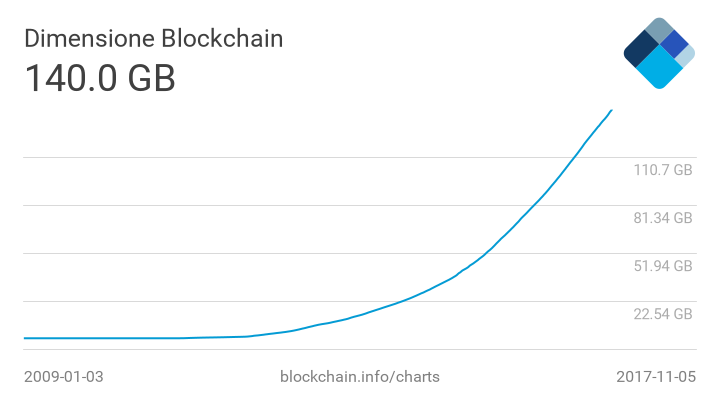
\includegraphics[width=0.8\textwidth]{blocks-size.png}
					\caption[Dimensione della blockchain di Bitcoin]{Dimensione della blockchain di Bitcoin.}
					\label{fig:blocks.size}
				\end{figure}
				\item \textbf{Adattabilità} - al momento la sola implementazione largamente diffusa della tecnologia la si trova in Bitcoin. Sebbene le sperimentazioni a riguardo siano innumerevoli, la necessità di fornire una ricompensa appetibile ha finora vincolato il successo delle proposte all'uso di tokenized blockchain. Nonostante queste si adattino straordinariamente bene all'ambito economico o alle operazioni di notariato, finora una flessibilità come quella della piattaforma Hyperledger rimane prerogativa dei sistemi non trustless;
				\item \textbf{Regolamentazione} - la rapida ascesa di blockchain non è seguita altrettanto rapidamente da una regolamentazione efficace dal punto di vista normativo. Tale regolamentazione si presenta come particolarmente problematica per via della natura libera, indipendente e incensurabile dei sistemi in questione;
				\item \textbf{Privacy} - diffondere copie dei registri attraverso la rete pone problemi non indifferenti per la riservatezza delle informazioni, su diversi livelli. Un primo aspetto, proprio di Bitcoin, è la pseudonimità del protocollo. Gli indirizzi con cui si opera nella rete sono infatti pubblici, ed è possibile risalire alla completa storia delle transazioni di un indirizzo. Esistono strategie più o meno efficaci per offuscare questo genere di informazioni, come sfruttare più indirizzi generati algoritmicamente invece di utilizzarne solamente uno o usare servizi come CoinJoin che permettono di accorpare transazioni di più utenti in maniera da rendere difficilmente tracciabile il flusso singolo di pagamento. Tuttavia, nel momento in cui si riuscisse ad associare l'indirizzo all'ente a cui è legato (impresa tutt'altro che proibitiva, dal momento che l'ente stesso deve diffondere l'indirizzo per utilizzarlo) la riservatezza delle transazioni sarebbe completamente compromessa. Un altro punto delicato riguarda la presenza di dati on-chain: anche se cifrati, questi sono infatti bloccati dall'immutabilità della blockchain. Ne consegue direttamente che un attacco a forza bruta su questi dati sarebbe facilitato di molto dall'impossibilità di modificare la chiave di cifratura dopo un certo periodo di tempo, vincolando la privacy su tali dati ad una inevitabile ``data di scadenza"; 
				\item \textbf{Impossibilità di interventi correttivi} - è un aspetto fortemente legato alla regolamentazione dei sistemi blockchain. L'immutabilità del registro, così come la completa assenza di governance da parte di un ente verificatore, comporta il fatto che una volta immessi dati o stabiliti dei contratti questi siano completamente fuori dal controllo di chiunque. È celebre l'incidente avvenuto con ``The DAO" sulla piattaforma Ethereum \cite{theDAO}, in cui uno smart contract mal formulato ha portato ad un attacco per un valore di circa 50 milioni di dollari. È estremamente difficile proteggere il sistema da evenienze di questo tipo senza rompere le fondamenta stesse su cui si basa: la protezione dell'utente in tali scenari è responsabilità esclusiva dell'utente stesso. Un esempio analogo lo si trova in Bitcoin, dove nel caso di perdita della chiave privata associata al proprio portafoglio si perde irrevocabilmente l'accesso ad esso e, dualmente, un malintenzionato che entrasse in possesso di un portafoglio ne potrebbe disporre a sua assoluta discrezione;
				\item \textbf{Rischio di Lock-in} - la resistenza alle modifiche dei sistemi basati su blockchain comporta delle situazioni indesiderabili per la sua adozione in produzione a livello aziendale. Un esempio è l'elevata dipendenza dalla specifica tecnologia adottata: la migrazione dei dati tra diverse blockchain è molto difficoltosa e, ricordando che ciò che garantisce la correttezza dei dati è la loro completa tracciabilità, interrompere la catena migrando da un sistema all'altro avrebbe gli stessi effetti descritti parlando del \hyperref[pruning]{\emph{pruning}} (sezione \ref{pruning}) rendendo violabile il sistema. Una soluzione possibile sarebbe permettere alla catena in cui si migra di ``puntare" alla catena precedente, tuttavia ciò frammenterebbe le garanzie di affidabilità del sistema e un fallimento di un singolo frammento di catena la comprometterebbe nella sua interezza;
				\item \textbf{Protezione dei wallet} - i problemi di scalabilità a cui si fa riferimento precedentemente comportano che l'utente del sistema si carichi di un onere considerevole in termini di memoria e risorse computazionali. Una soluzione spesso adottata è quella di affidarsi a wallet esterni: si tratta di nodi completi, gestiti da un intermediario, che espongono le funzionalità di base agli utenti esterni. Questo si rivela un enorme rischio per la sicurezza in quanto ogni client deve necessariamente riporre un forte trust nei confronti del wallet, rendendo spesso completamente superfluo l'impiego di un sistema blockchain. Inoltre, nell'analizzare la sicurezza generale del sistema bisogna considerare che il punto più fragile potrebbe essere proprio questo intermediario. È necessario perciò disincentivare quanto più possibile tale pratica, preoccupandosi di fornire agli utenti informazioni chiare a riguardo e dotandoli di un sistema non eccessivamente oneroso da sostenere;
				\item \textbf{Sybil attack} - un possibile attacco ad un sistema blockchain vede un eventuale attaccante tentare di saturare il network con nodi malevoli, in modo che sia altamente probabile che un utente si connetta solo a peer compromessi. Questa situazione può essere sfruttata in diversi modi, tra cui i seguenti:
				\begin{itemize}
					\item L'attaccante può bloccare la propagazione delle informazioni da parte del resto della rete, isolando i nodi che dipendono da quelli compromessi;
					\item L'attaccante può inoltrare solo blocchi da lui creati, creando un fork artificiale della blockchain non verificabile da parte dei nodi isolati e aprendo alla possibilità di double-spending;
					\item Anche senza passare per il punto illustrato al passo precedente, se il client fa affidamento su transazioni senza richiedere più livelli di ``profondità" del blocco per ritenerle confermate è vulnerabile a double-spending;
					\item Sistemi di anonimizzazione a bassa latenza come quelli utilizzati tipicamente dai client Bitcoin (e.g. Tor) possono essere rotti facilmente con dei \emph{timing attack} qualora l'attaccante avesse un controllo sulla rete come quello descritto;
				\end{itemize}
				\item \textbf{Majority attack} - qualora un attaccante avesse il controllo della maggior parte del ``potere di consenso" nella rete (potenza di calcolo nel caso di proof-of-work, valuta nel caso di proof-of-stake, etc.) potrebbe effettuare double spending creando un fork della blockchain. In seguito potrebbe far crescere la catena compromessa a velocità maggiore di quella ufficiale fino a renderla la catena più lunga, e quindi quella accettata dalla rete;
				\item \textbf{Flood attack} - un attaccante potrebbe inviare ripetutamente transazioni a se stesso, saturando la capienza massima del blocco e impedendo alle altre transazioni di essere elaborate. Bitcoin contrasta attacchi di questo tipo limitando le transazioni gratuite per blocco a 50KB, per cui tale attaccante esaurito lo spazio gratuito dovrebbe pagare una commissione che renderebbe l'attacco costoso, tuttavia in un sistema generico che volesse essere completamente gratuito questa potrebbe essere una vulnerabilità presente;
				\item \textbf{Timejacking attack}\cite{timejacking} - questo tipo di vulnerabilità è peculiare di Bitcoin e dipende da alcune sue caratteristiche specifiche, tuttavia è citata per far comprendere quanto delicati siano gli algoritmi sottostanti ai sistemi blockchain. Ogni nodo del sistema mantiene un contatore interno che rappresenta il \emph{tempo di rete}, necessario per determinare fattori come la validità dei blocchi o il tempo medio di validazione necessario al calcolo della ``difficoltà" del blocco successivo. Un attaccante potrebbe velocizzare o rallentare questo contatore attraverso ripetute connessioni al nodo comunicando timestamp alterati. Grazie alla discrepanza su questo contatore e al fatto che Bitcoin scarta automaticamente blocchi con timestamp che diverge troppo da quello interno, è possibile provocare un fork della catena e aprire a possibilità di double spending, come spiegato in dettaglio nell'articolo in nota.
			\end{itemize}
